\documentclass[8pt]{article}
\usepackage[top=0.2in, bottom=0.2in, left=0.2in, right=0.2in]{geometry} % Adjust margins individually
\usepackage{amsmath,amssymb,amsthm}
\usepackage{enumitem}
\usepackage{graphicx} % Required for \includegraphics
\usepackage{ragged2e}

\usepackage[absolute,overlay]{textpos}
\usepackage{array} % For better column definitions
\usepackage{booktabs} % For improved table aesthetics
\raggedbottom
\setlist[itemize]{leftmargin=0mm}
\newcommand{\dist}[2]{\left\langle #1,\, #2 \right\rangle}
\setlength{\TPHorizModule}{0.1mm} % Set horizontal units to millimeters
\setlength{\TPVertModule}{0.1mm}  % Set vertical units to millimeters
\usepackage{multicol}
\setlength{\parindent}{0pt}
\setlength{\parskip}{5pt plus 1pt minus 1pt}
\usepackage{setspace}
\setstretch{1}
\pagestyle{empty}

% Redefine the textblock environment
\let\originaltextblock\textblock
\let\endoriginaltextblock\endtextblock

\renewenvironment{textblock}[2][]{%
    \originaltextblock[#1]{#2}%
    \fcolorbox{red}{white}{%
    \begin{minipage}{#2}%
}{%
    \end{minipage}%
    }%
    \endoriginaltextblock
}


\begin{document}
\begin{titlepage}
    \centering
    \vspace*{1cm}
    {\Huge \textbf{Analysis III - CheatSheet}} \\
    \vspace{10px}
    {\LARGE IN~BA3 - Martin Werner Licht} \\
    \vspace*{1cm}
    {\Large Notes by Ali EL AZDI} \\
    \vfill

    \begin{justify}
        \textit{An Analysis III Cheatsheet has been authorized for the upcoming exam, and I’m sharing a copy of mine for anyone interested. It provides a concise summary of the key concepts and techniques covered in the course. While it’s not yet complete, I plan to update it soon, especially to include additional trigonometric identities and a step-by-step guide to solving differential equations using Fourier methods. When printing, you can select the last two pages, as only one A4 recto-verso page is allowed. For any updates or suggestions, feel free to reach out to me on Telegram at \texttt{elazdi\_al} or via EPFL email at \texttt{ali.elazdi@epfl.ch}.}
    \end{justify}
    \vspace*{100px}

    {\large January 3rd, 2025}
    \vspace*{20px}
\end{titlepage}


\vspace*{-10px}
\noindent\textbf{Regular Curve.}
A continuously differentiable map
$\gamma : [a,b] \to \mathbb{R}^n$
is \emph{regular} if $\gamma'(t) \neq 0$ for all $t \in [a,b]$.

\smallskip
\noindent\textbf{Simple Curve.}
A continuous map
$\gamma : [a,b] \to \mathbb{R}^n$
is \emph{simple} if it does not intersect itself (except possibly at endpoints):
$\gamma(t_1) = \gamma(t_2) \implies t_1 = t_2$

\smallskip
\noindent\textbf{Simply Connected Domain.}
An open set $\Omega \subseteq \mathbb{R}^n$ is \emph{simply connected} if for any two continuous curves
$\gamma_0, \gamma_1 : [a,b] \to \Omega$
with $\gamma_0(a) = \gamma_1(a)$ and $\gamma_0(b) = \gamma_1(b)$,
there exists a continuous homotopy
$\Gamma : [a,b]\times[0,1] \to \Omega$
that deforms $\gamma_0$ into $\gamma_1$ within $\Omega$ while keeping the endpoints fixed.
\smallskip \newline
\noindent\textbf{Curve in } $\mathbb{R}^n$: Given $\gamma : [a,b] \to \mathbb{R}^n$,$ \int_{\gamma} F \cdot d\mathbf{l} = \int_a^b \big\langle F(\gamma(t)), \gamma'(t)\big\rangle \, dt, \quad \int_{\gamma} f(\mathbf{x}) \, ds = \int_a^b f\big(\gamma(t)\big)\,\|\gamma'(t)\| \, dt.$\\
\noindent\textbf{Surface in } $\mathbb{R}^3$:
Given $\sigma : D \subset \mathbb{R}^2 \to \mathbb{R}^3$, $\sigma(u,v)$, \vspace{-10px}
\[
\iint_{\sigma} F \cdot d\mathbf{S}
= \iint_D \big\langle F(\sigma(u,v)), \sigma_u(u,v)\times\sigma_v(u,v)\big\rangle \,du\,dv.
\quad
\iint_{\sigma} f(\mathbf{x}) \, ds
= \iint_D f\big(\sigma(u,v)\big)\,\|\sigma_u(u,v)\times\sigma_v(u,v)\| \,du\,dv,
\]
\noindent \textbf{Conservative Fields and Path Independence}\\
A map \( F : \Omega \subseteq \mathbb{R}^n \to \mathbb{R}^n \) is \emph{conservative} if there exists a differentiable function \( \varphi : \Omega \to \mathbb{R} \) such that \( \nabla f = F \).\\
\small
$
F \text{ is conservative on } \Omega \; \iff \;
\forall \Gamma_1, \Gamma_2 \subseteq \Omega \text{ reg. curves from } A \text{ to } B, \; \int_{\Gamma_1} F \cdot \, d\mathbf{l} = \int_{\Gamma_2} F \cdot \, d\mathbf{l}, \;
\iff \; \forall \Gamma \subseteq \Omega \text{ reg. closed curve}, \; \int_{\Gamma} F \cdot \, d\mathbf{l} = 0.
$\\
\normalsize
\noindent\textbf{is $\mathbf{F}$ Conservative over $\Omega$ ?}\newline
\begin{minipage}[t]{0.17\textwidth}
    \noindent\textbf{1 - Compute $\operatorname{curl} \mathbf{F}$.} \vspace{-8px}
    \begin{itemize}[leftmargin=*]
        \setlength\itemsep{-4px}
        \item[-] If $\operatorname{curl} \mathbf{F} \neq \mathbf{0}$, $\mathbf{F}$ is \textbf{not} conservative.
        \item[-] If $\operatorname{curl} \mathbf{F} = \mathbf{0}$, proceed to Step 2.
    \end{itemize}
\end{minipage}
\hfill
\begin{minipage}[t]{0.25\textwidth}
    \noindent\textbf{2 - is $\Omega$ Simply Connected ?} \vspace{-8px}
    \begin{itemize}[leftmargin=*]
        \setlength\itemsep{-4px}
        \item[-] If \textit{yes}, $\mathbf{F}$ is conservative.
        \item[-] If \textit{no}, proceed to Step 3.
    \end{itemize}
\end{minipage}
\hfill
\begin{minipage}[t]{0.23\textwidth}
    \noindent\textbf{3 - Circulation Method:} \vspace{-8px}

    \begin{enumerate}[leftmargin=*]
        \setlength\itemsep{-4px}
        \item Select closed curves $\Gamma$ around each hole in $\Omega$.
        \item Compute $\oint_{\Gamma} \mathbf{F} \cdot d\mathbf{l}$.
        \item If any integral $\neq 0$, $\mathbf{F}$ is \textbf{not} conservative.
        \item If all integrals $=0$, proceed to Step 4.
    \end{enumerate}
\end{minipage}
\hfill
\begin{minipage}[t]{0.29\textwidth}
    \noindent\textbf{4 - Finding the Potential} \vspace{-8px}
    \[
        \varphi(x,y,z) = \int_{x_0}^x F_1(t,y,z) \, dt + \alpha(y,z)
    \] \vspace{-25px}

    \begin{enumerate}[leftmargin=*]
        \setlength\itemsep{-4px} % Reduces spacing even further
        \item Determine $\alpha(y,z)$ such that \\ $\nabla \varphi = \mathbf{F}$.
        \item If successful, $\varphi$ is the potential function for $\mathbf{F}$, confirming $\mathbf{F}$ is conservative.
    \end{enumerate}

\end{minipage}
\vspace*{-30px}
\subsubsection*{Vector Calculus Theorems}
\begin{minipage}[htp]{0.49\textwidth}
\noindent\textbf{Green's Theorem (Plane)}
Let \( \Omega \subseteq \mathbb{R}^2 \) be a regular domain with a positively oriented boundary \( \partial \Omega \), and \( F \in C^1(\overline{\Omega}, \mathbb{R}^2) \). Then
\vspace{-10px}\[
\iint_{\Omega} \operatorname{curl}(F(x, y)) \, dx \, dy = \int_{\partial \Omega} F \cdot dl
\]
\end{minipage}
\hfill
\begin{minipage}[htp]{0.49\textwidth}
\noindent\textbf{Divergence Theorem (Plane)}
Let \( \Omega \subseteq \mathbb{R}^2 \) be a regular domain with a positively oriented boundary \( \partial \Omega \), and \( F \in C^1(\overline{\Omega}, \mathbb{R}^2) \). Then
\vspace{-10px}\[
\iint_{\Omega} \operatorname{div} F(x, y) \, dx \, dy = \int_{\partial \Omega} F \cdot n \, dl = \int_a^b \left\langle F(\gamma(t)), (\gamma_2'(t), -\gamma_1'(t)) \right\rangle dt.
\]\vspace{-10px}
\end{minipage}
\\
\begin{minipage}[htp]{0.49\textwidth}
\noindent\textbf{Divergence Theorem (Space)}
Let \( \Omega \subseteq \mathbb{R}^3 \) be a regular domain, \( n : \partial \Omega \to \mathbb{R}^3 \) a continuous outward unit normal vector field, and \( F \in C^1(\overline{\Omega}, \mathbb{R}^3) \). Then
\[
\iiint_{\Omega} \operatorname{div} F(x,y,z) \, dx \, dy \, dz = \iint_{\partial \Omega} F \cdot n \, ds = \iint_{A} \langle F(\sigma(u,v)); \frac{\partial \sigma}{\partial u}(u,v) \wedge \frac{\partial \sigma}{\partial v}(u,v) \rangle \, du \, dv
\]

\end{minipage}
\hfill
\begin{minipage}[htp]{0.49\textwidth}
\noindent\textbf{Stokes' Theorem}
Let \( \Omega \subseteq \mathbb{R}^3 \) be an open set, \( \Sigma \subseteq \Omega \) a piecewise smooth orientable surface, and \( F \in C^1(\Omega, \mathbb{R}^3) \), then
\vspace{-10px}\[
\iint_{\Sigma} \operatorname{curl} F \, ds = \int_{\partial \Sigma} F \cdot dl
\]
\end{minipage}\\
\begin{minipage}[t]{0.27\textwidth}
    \centering
  \noindent  \textbf{Polar (2D)} \\[4pt]
    \(|\det J| = r\) \\[4pt]
    \(\displaystyle
    \begin{bmatrix}
    x \\[4pt]
    y
    \end{bmatrix}
    =
    \begin{bmatrix}
    r\cos\theta \\[4pt]
    r\sin\theta
    \end{bmatrix};
    \) \\[4pt]
    \( r \geq 0, \; \theta \in [0, 2\pi] \).
\end{minipage}
\hfill
\begin{minipage}[t]{0.27\textwidth}
    \centering
    \textbf{Cylindrical (3D)} \\[4pt]
    \(|\det J| = r\) \\[4pt]
    \(\displaystyle
    \begin{bmatrix}
    x \\[4pt]
    y \\[4pt]
    z
    \end{bmatrix}
    =
    \begin{bmatrix}
    r\cos\theta \\[4pt]
    r\sin\theta \\[4pt]
    z
    \end{bmatrix};
    \) \\[4pt]
    \( r \geq 0, \; \theta \in [0, 2\pi), \; z \in (-\infty, \infty) \).
\end{minipage}
\hfill
\begin{minipage}[t]{0.37\textwidth}
    \centering
    \textbf{Spherical (3D)} \\[4pt]
    \(|\det J| = \rho^2\sin\phi\) \\[4pt]
    \(\displaystyle
    \begin{bmatrix}
    x \\[4pt]
    y \\[4pt]
    z
    \end{bmatrix}
    =
    \begin{bmatrix}
    \rho\sin\phi\cos\theta \\[4pt]
    \rho\sin\phi\sin\theta \\[4pt]
    \rho\cos\phi
    \end{bmatrix};
    \) \\[4pt]
    \( \rho \geq 0, \; \phi \in [0, \pi], \; \theta \in [0, 2\pi] \).
\end{minipage}

\noindent \textbf{Distribution Theory} \\
Let $\mathcal{D}'$ be the set of distributions over $\mathbb{R}$, the set of linear continuous functionals over $\mathcal{D}$,
$
\mathcal{D}' = \left\{ T \colon \mathcal{D} \to \mathbb{R} \;\middle|\; T \text{ is linear and continuous} \right\}.
$\\
For a distribution $T \in \mathcal{D}'$ and a test function $\varphi \in \mathcal{D}$, the pairing is defined by
$
\langle T, \varphi \rangle = \int_{\Omega} f(x) \varphi(x) \, dx.
$
\\
A distribution $T \in \mathcal{D}'$ satisfies: \vspace{-13px}\hspace{170px}\fbox{%
\begin{minipage}[t]{0.25\textwidth}
    \textbf{Support}\\
    \vspace{-10px}
    \[
    \mathrm{supp}(T)
    = \overline{\{\, x \in \mathbb{R} \mid T(\varphi) \neq 0 \}}.
    \]
\end{minipage}
}
\fbox{%
    \begin{minipage}[t]{0.18\textwidth}
        \textbf{Derivative} \\
        $\varphi \in \mathcal{D}$, $T'(\varphi) = -T(\varphi').$ \\
        \vspace{-1em} % Reduces vertical space after the second line
    \end{minipage}
}\\ \vspace{-5px}

\noindent \textbf{Boundedness} For every $\psi \in \mathcal{D}$, $|T(\psi)|$ is finite. \\
\noindent \textbf{Linearity} For all scalars $\alpha, \beta \in \mathbb{R}$ and test functions $\psi, \varphi \in \mathcal{D}$,
    $
    T(\alpha \psi + \beta \varphi) = \alpha T(\psi) + \beta T(\varphi).
    $ \\
\noindent \textbf{Continuity} \\ \noindent\makebox[\textwidth][l]{$ \forall [a, b] \subseteq \mathbb{R}$, there exist constants $C > 0$ and $k \in \mathbb{N}_0$, such that $\forall \varphi \in \mathcal{D}$, $\text{supp}(\varphi) \subseteq [a, b] \implies \left| T(\varphi) \right| \leq C \sum_{0 \leq i \leq k} \max_{x \in \mathbb{R}} \left| \partial^i \varphi(x) \right|.$}
\noindent \textbf{Higher-Order Derivatives} $\forall n \in \mathbb{N}$, $T^{(n)}(\varphi) = (-1)^n T(\varphi^{(n)})$. \\ \vspace*{-30px}
\noindent
\begin{minipage}[t]{0.24\textwidth}
    \textbf{Dirac Delta}\\
    $\delta(\varphi) = \varphi(0)$ for all $\varphi \in \mathcal{D}.$\\ \smallskip \\
    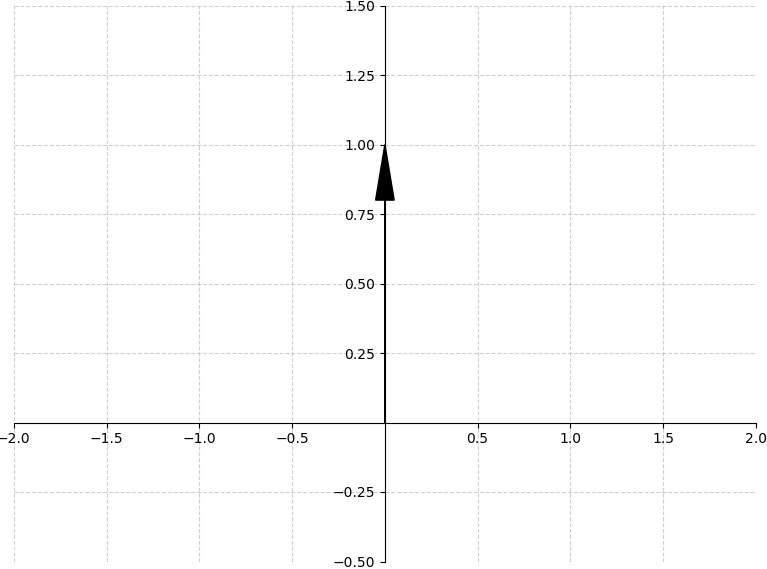
\includegraphics[width=1.05\linewidth]{images/dirac_delta.png}
\end{minipage}
\hfill
\begin{minipage}[t]{0.24\textwidth}
    \textbf{Dirac Comb}\\
    $\Delta_T(x) = \sum_{n \in \mathbb{Z}} \delta(x - nT),$\\
    $T > 0$ is the period.\smallskip \\
    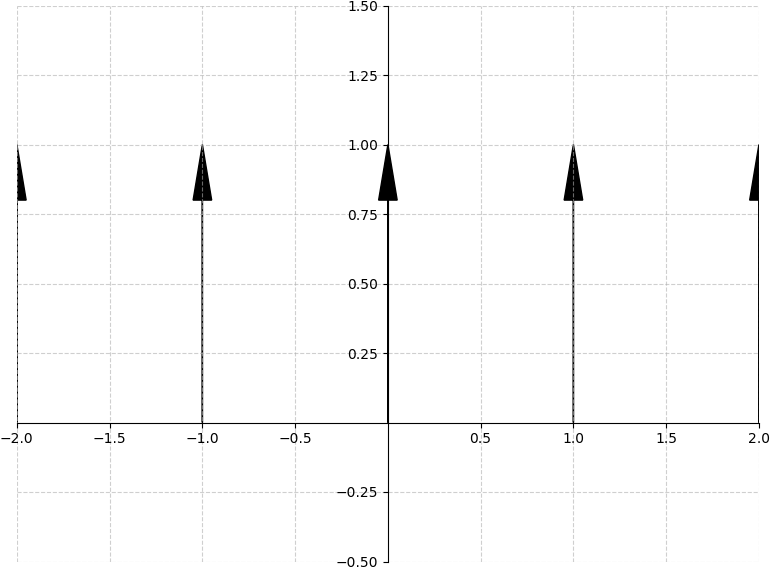
\includegraphics[width=1.05\linewidth]{images/dirac_comb.png}
\end{minipage}
\hfill
\begin{minipage}[t]{0.24\textwidth}
    \textbf{Scaled Dirac Delta}\\
    $a \in \mathbb{R}$, $(a\delta)(\varphi) = a \cdot \varphi(0).$ \smallskip \\\\
    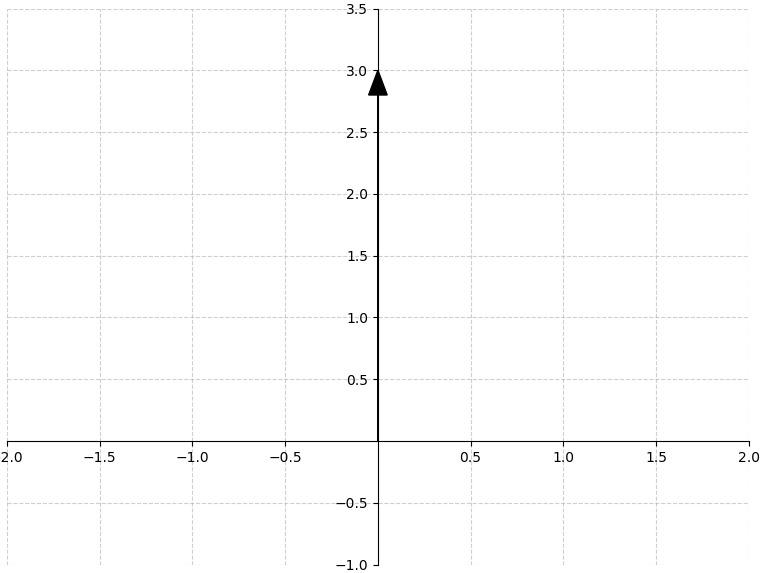
\includegraphics[width=1.05\linewidth]{images/scaled_dirac_delta.png}
\end{minipage}
\hfill
\begin{minipage}[t]{0.24\textwidth}
    \textbf{Heaviside Step}\\
    $H(x) =
    \begin{cases}
      0 & \text{if } x < 0,\\
      1 & \text{if } x \geq 0.
    \end{cases}$ \\
    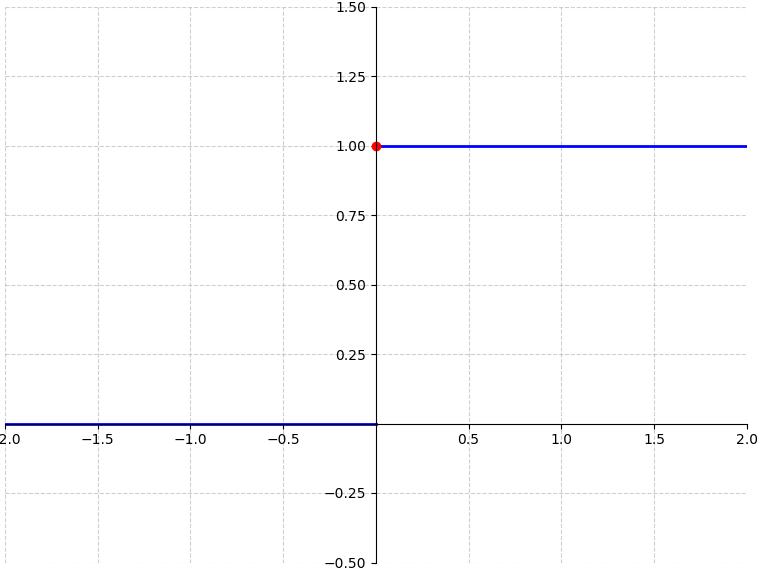
\includegraphics[width=1.05\linewidth]{images/heaviside.png}
\end{minipage}
% Reduce paragraph spacing/indentation:
\setlength{\parindent}{0pt}
\setlength{\parskip}{0pt}



\footnotesize  % Slightly smaller font to fit all content comfortably

\begingroup
% ----------------------------------------------------------------------
% Adjust spacing for displayed equations:
\setlength{\abovedisplayskip}{3pt}
\setlength{\belowdisplayskip}{3pt}
\setlength{\abovedisplayshortskip}{2pt}
\setlength{\belowdisplayshortskip}{2pt}

% Adjust spacing for itemize/enumerate:
\let\oldenumerate\enumerate
\def\enumerate{\oldenumerate
  \setlength{\itemsep}{0pt}
  \setlength{\parskip}{0pt}
  \setlength{\parsep}{0pt}
}
\let\olditemize\itemize
\def\itemize{\olditemize
  \setlength{\itemsep}{0pt}
  \setlength{\parskip}{0pt}
  \setlength{\parsep}{0pt}
}
\setstretch{0.6}
% ----------------------------------------------------------------------
\small
\begin{multicols}{2}

\noindent \textbf{Piecewise Continuity \& Differentiability}\\
$f:[a,b]\to\mathbb{R}$ is \emph{piecewise continuous} if there is a partition
\[
  a=a_0 < a_1 < \dots < a_n = b
\]
such that $\lim_{x \to a_i^-} f(x)$ and $\lim_{x \to a_i^+} f(x)$ exist (finite).\\
Similarly, $f$ is \emph{piecewise $C^1$} if it is continuously differentiable on each open subinterval and the one‐sided derivatives at boundaries exist.\\

\noindent \textbf{Euler's Formulas}
\[
  e^{x+iy} = e^{x}\bigl(\cos y + i \sin y\bigr),\;
  \sin x = \frac{e^{ix}-e^{-ix}}{2i},\;
  \cos x = \frac{e^{ix}+e^{-ix}}{2}.
\]

\noindent \textbf{Orthogonality (Sine/Cosine Products)}\\
For $n,m \in \mathbb{N}_{\ge 1}$ and period $T>0$:
\[
  \frac{2}{T} \int_{0}^{T}
  \cos\!\Bigl(\tfrac{2\pi n}{T}x\Bigr)\cos\!\Bigl(\tfrac{2\pi m}{T}x\Bigr)\,dx
=
\begin{cases}
1 & n=m,\\
0 & n\neq m
\end{cases}
\]
(Same for $\sin\sin$, and $\cos\sin$ integrates to $0$.)\\

\noindent \textbf{Integration Over One Period}\\
If $f$ is $T$-periodic and piecewise continuous, then for any $a\in\mathbb{R}$:
\[
  \int_{a}^{a+T} f(x)\,dx = \int_{0}^{T} f(x)\,dx.
\]

\noindent \textbf{Dirichlet's Theorem (Pointwise Convergence)}\\
Let \( f : \mathbb{R} \to \mathbb{R} \) be \( T \)-periodic and piecewise \( C^1 \). Then, for all \( x \in \mathbb{R} \),
\[
  Ff(x) = \lim_{t \to 0} \frac{f(x - t) + f(x + t)}{2}.
\]

\noindent \textbf{Real Fourier Series}\\
For $f:\mathbb{R}\to\mathbb{R}$, $T$-periodic, piecewise $C^1$, the real Fourier series is
\[
  Ff(x)= \frac{a_{0}}{2}
   + \sum_{n=1}^{\infty}\!\Bigl[a_{n}\cos\!\bigl(\tfrac{2\pi n}{T}x\bigr)
   + b_{n}\sin\!\bigl(\tfrac{2\pi n}{T}x\bigr)\Bigr].
\]
\noindent \textbf{Fourier Coefficients:}
\[
  a_{n} = \frac{2}{T}\!\int_{0}^{T}\!f(x)
          \cos\!\Bigl(\tfrac{2\pi n}{T}x\Bigr)\,dx,\quad
  b_{n} = \frac{2}{T}\!\int_{0}^{T}\!f(x)
          \sin\!\Bigl(\tfrac{2\pi n}{T}x\Bigr)\,dx,
\]
\[
  a_{0} = \frac{2}{T}\int_{0}^{T} f(x)\,dx.
\]
\noindent \textbf{Parity:} If $f$ is even, $b_{n}=0$; if $f$ is odd, $a_{n}=0$.\\

\small
\noindent \textbf{Convolution Product}\\
Let \(f,g:\mathbb{R} \to \mathbb{R}\) such that
\(\int_{-\infty}^{+\infty} |f(x)|\,dx < +\infty\) and
\(\int_{-\infty}^{+\infty} |g(x)|\,dx < +\infty\).
\[
  (f * g)(x)
  = \int_{-\infty}^{+\infty} f(x - t)\,g(t)\,dt
  = \int_{-\infty}^{+\infty} f(t)\,g(x - t)\,dt
\]
\noindent \textbf{Term-by-Term Differentiation}\\
If $f$ is $T$-periodic, continuous, and piecewise $C^1$, then
\[
  \frac{d}{dx}\bigl[Ff(x)\bigr]
  = \sum_{n=1}^\infty \frac{2\pi n}{T}\bigl[-\,a_n\sin(\tfrac{2\pi n}{T}x)
    +b_n\cos(\tfrac{2\pi n}{T}x)\bigr]
\]
\[
  = \lim_{t \to 0} \frac{f'(x - t) + f'(x + t)}{2}.
\]

\noindent \textbf{1) Poisson on }$[a,b]$:
\[
\begin{cases}
-\,u''(x)=f(x),\\[2pt]
u(a)=g_a,\quad u(b)=g_b,
\end{cases}
\quad
L = b - a
\]
\[
u^g(x)=\frac{g_b-g_a}{b-a}\,x \;+\;\frac{b\,g_a - a\,g_b}{b-a}.
\]
\[
f(x)=\sum_{n=1}^{\infty} b_n \,\sin\!\Bigl(\frac{n\pi x}{L}\Bigr),
\quad
b_n=\frac{2}{L}\int_{0}^{L}f(t)\,\sin\!\Bigl(\frac{n\pi t}{L}\Bigr)\,dt,
\]
\[
u^f(x)=\sum_{n=1}^{\infty} b_n \,\frac{L^2}{\pi^2\,n^2}
\,\sin\!\Bigl(\frac{n\pi x}{L}\Bigr).
\]
\[
u(x)=u^g(x)+u^f(x).
\]
\noindent \textbf{2) Poisson with mass term on }$\mathbb{R}$:
\[
-\,u''(x)+k^2\,u(x)=f(x),
\quad
\widehat{u}(\alpha)=\frac{\widehat{f}(\alpha)}{\alpha^2 + k^2}.
\]
\[
g(x)=\frac{1}{2k}\,e^{-k|x|},
\quad
\widehat{g}(\alpha)=\frac{1}{\alpha^2 + k^2},
\quad
u(x)=(g*f)(x)
=\frac{1}{2k}\!\int_{-\infty}^{\infty} f(y)\,e^{-k|\,x-y\,|}\,dy.
\]

\columnbreak

\noindent \textbf{Complex Fourier Coefficient}\\
Let \( f : \mathbb{R} \to \mathbb{R} \) be \( T \)-periodic and piecewise continuous.  The complex Fourier coefficients are:
\[
  c_n = \frac{1}{T} \int_0^T f(x)\, e^{-i \frac{2\pi}{T} n x} \, dx,
  \quad
  Ff(x) = \sum_{n=-\infty}^{\infty} c_{n}\,e^{i\frac{2\pi n}{T}x}.
\]
For \( \phi : \mathbb{R} \to \mathbb{C} \),
\[
  \int_a^b \phi(x)\,dx
  = \int_a^b \operatorname{Re}(\phi(x)) \, dx + i \int_a^b \operatorname{Im}(\phi(x)) \, dx.
\]
\noindent \textbf{Relation to \( (a_n, b_n) \)}\quad
\[
  c_{n} = \tfrac{1}{2}(a_{n} - i\,b_{n}),\
  c_{-n} = \tfrac{1}{2}(a_{n} + i\,b_{n}),\
  c_{0} = \tfrac{a_{0}}{2}.
\]

\noindent \textbf{Fourier Series on $[0,L]$}\\
For $f:[0,L]\to \mathbb{R}$ (piecewise $C^1$):
\[
  F_{c}f(x)=\tfrac{\tilde a_{0}}{2} + \sum_{n=1}^{\infty}\!\tilde a_{n}\cos\!\Bigl(\tfrac{\pi n}{L}x\Bigr),
  \quad \tilde a_{n}=\frac{2}{L}\int_{0}^{L} f(x)\cos\!\Bigl(\tfrac{\pi n}{L}x\Bigr)\,dx.
\]
\[
  F_{s}f(x)=\sum_{n=1}^{\infty}\!\tilde b_{n}\sin\!\Bigl(\tfrac{\pi n}{L}x\Bigr),
  \quad \tilde b_{n}=\frac{2}{L}\int_{0}^{L} f(x)\sin\!\Bigl(\tfrac{\pi n}{L}x\Bigr)\,dx.
\]

\noindent \textbf{Parseval's Identity (Periodic Case)}\\
If $f$ is $T$-periodic (piecewise $C^1$),
\[
  \frac{2}{T}\int_{0}^{T} f^{2}(x)\,dx
  = \frac{a_{0}^{2}}{2} + \sum_{n=1}^{\infty}(a_{n}^{2}+b_{n}^{2})
  = 2\sum_{n=-\infty}^{\infty}\!\!\bigl|c_{n}\bigr|^{2}.
\]

\noindent \textbf{Plancherel Theorem}\\
Let $f \in L^2(\mathbb{R})$. Then its Fourier transform $\hat{f}$ is also in $L^2(\mathbb{R})$, and:
\[
  \int_{-\infty}^\infty |f(x)|^2 \, dx
  = \int_{-\infty}^\infty |\hat{f}(\xi)|^2 \, d\xi.
\]

\noindent \textbf{The Fourier Transform}\\
If $f:\mathbb{R}\to\mathbb{R}$ with $\int_{-\infty}^{\infty}\!|f(x)|\,dx<\infty$, its (unitary) Fourier transform is
\[
  \widehat{f}(\alpha)=\frac{1}{\sqrt{2\pi}}
  \int_{-\infty}^{\infty} f(x)\, e^{-\,i\,\alpha x}\,dx,
\]
\noindent \textbf{Inverse Transform}\\
If $\varphi(\alpha)$ is similarly integrable,
\[
  \mathcal{F}^{-1}(\varphi)(x)= \frac{1}{\sqrt{2\pi}}
  \int_{-\infty}^{\infty}\!\varphi(\alpha)\,e^{\,i\,\alpha x}\,d\alpha.
\]

\noindent \textbf{Fourier Transform of \(f * g\)}\\
Let \(f\) and \(g\) be piecewise continuous and absolutely integrable. Then
\[
  \int_{-\infty}^{+\infty} |(f * g)(x)|\,dx < +\infty,\quad
  \mathcal{F}[f * g](\alpha)
  = \sqrt{2\pi} \,\hat{f}(\alpha)\,\hat{g}(\alpha).
\]
\vspace*{-15px}
\setlength{\columnsep}{-35pt} % Slight negative shift to fit columns nicely
\begin{multicols}{2}
    \small
    \textbf{Scaling} \\
    $\mathcal{F}\{f(ax)\} = \frac{1}{|a|} F\!\bigl(\tfrac{\alpha}{a}\bigr)$\\
    \textbf{Shifting} \\
    $\mathcal{F}\{f(x - x_0)\} = e^{-\,i\,\alpha x_0}\,F(\alpha)$\\
    \textbf{Modulation} \\
    $\mathcal{F}\{e^{\,i\,\omega_0 x} f(x)\} = F(\alpha - \omega_0)$\\
    \textbf{Differentiation} \\
    $\mathcal{F}\!\Bigl\{\dfrac{d^n}{dx^n}f(x)\Bigr\}
        = (i \alpha)^n F(\alpha)$\\


    \columnbreak

    \textbf{Integration} \\
    $\mathcal{F}\!\Bigl\{\int_{-\infty}^x f(\xi)\,d\xi\Bigr\}
        = \dfrac{1}{i \alpha}\,F(\alpha),\ \alpha\neq 0$
    \textbf{Multiplication} \\
    $\mathcal{F}\{f(x)\,g(x)\}(\alpha)
      = \dfrac{1}{2\pi}\!\int_{-\infty}^{\infty}
        F(\kappa)\,G(\alpha - \kappa)\,d\kappa$\\
    \textbf{Real/Imag Parts} \\
    $\mathcal{F}\{\text{Re}[\,f(x)\,]\}
      = \dfrac{F(\alpha) + F^*(-\alpha)}{2}$,\\
      $\mathcal{F}\{\text{Im}[\,f(x)\,]\}
      = \dfrac{F(\alpha) - F^*(-\alpha)}{2i}$
\end{multicols}
\noindent \textbf{Important Trigonometric Identities} \\
$\sin(2x) = 2\sin x\cos x,$\\
$\cos(2x) = 2\cos^2 x - 1 = 1 - 2\sin^2 x = \cos^2 x - \sin^2 x,$\\
$\cos(a \pm b) = \cos a\cos b \mp \sin a\sin b,$\\
$\sin(a \pm b) = \sin a\cos b \pm \cos a\sin b.$\\
$\cos a\cos b = \tfrac{1}{2}\bigl[\cos(a - b) + \cos(a + b)\bigr],$ \\
$\sin a\sin b = \tfrac{1}{2}\bigl[\cos(a - b) - \cos(a + b)\bigr],$ \\
$\sin a\cos b = \tfrac{1}{2}\bigl[\sin(a + b) + \sin(a - b)\bigr],$ \\
$\cos a\sin b = \tfrac{1}{2}\bigl[\sin(a + b) - \sin(a - b)\bigr].$

\normalsize
\end{multicols}
\endgroup
\end{document}
